\subsection{Times Table} % (fold)
\label{sub:times_table}

This program prints out the times table for a number entered by the user, displaying from 1 x n to 10 x n. The description of the program is in Table \ref{tbl:data-times-table}, the pseudocode in Listing \ref{lst:data-times-pseudo}, the C code in Listing \ref{lst:data-times-c}, and the Pascal code in Listing \ref{lst:data-times-pas}.

\begin{table}[h]
\centering
\begin{tabular}{l|p{10cm}}
  \hline
  \multicolumn{2}{c}{\textbf{Program Description}} \\
  \hline
  \textbf{Name} & \emph{Times Table} \\
  \\
  \textbf{Description} & Displays the Times Table from 1 x n to 10 x n. \\
  \hline
\end{tabular}
\caption{Description of the Times Table program}
\label{tbl:data-times-table}
\end{table}

\pseudocode{lst:data-times-pseudo}{Pseudocode for Times Table program.}{./topics/storing-using-data/examples/times-table.txt}

\mynote{
This is an updated version of the Seven Times Table Program. See Section \ref{sub:seven_times_table} \nameref{sub:seven_times_table}.
}

\clearpage

\csection{\ccode{lst:data-times-c}{C Times Table}{topics/storing-using-data/examples/times_table.c}}

\passection{\pascode{lst:data-times-pas}{Pascal Times Table}{topics/storing-using-data/examples/TimesTable.pas}}

% subsection times_table (end)

\clearpage
\subsection{Circle Area} % (fold)
\label{sub:circle_area_data}

This program prints out the area of a circle. The description of the program is in Table \ref{tbl:data-circle-area}, the pseudocode in Listing \ref{lst:data-circle-areas-pseudo}, the C code in Listing \ref{lst:data-circle-areas-c}, and the Pascal code in Listing \ref{lst:data-circle-areas-pas}.

\begin{table}[h]
\centering
\begin{tabular}{l|p{10cm}}
  \hline
  \multicolumn{2}{c}{\textbf{Program Description}} \\
  \hline
  \textbf{Name} & \emph{Circle Areas} \\
  \\
  \textbf{Description} & Displays the Circle Areas for circles with radius from 1.0 to 5.0 with increments of 0.5. \\
  \hline
\end{tabular}
\caption{Description of the Circle Areas program}
\label{tbl:data-circle-area}
\end{table}

\pseudocode{lst:data-circle-areas-pseudo}{Pseudocode for Circle Areas program.}{./topics/storing-using-data/examples/circle_areas.txt}

\mynote{
This is an updated version of the Circle Areas Program. See Section \ref{sub:circle_area} \nameref{sub:circle_area}.
}


\clearpage

\csection{\ccode{lst:data-circle-areas-c}{C Circle Areas}{topics/storing-using-data/examples/circle_areas.c}}

\passection{\pascode{lst:data-circle-areas-pas}{Pascal Circle Areas}{topics/storing-using-data/examples/CircleAreas.pas}}

% subsection circle_area (end)
\clearpage
\subsubsection{Water Tank} % (fold)
\label{ssub:water_tank}

The \emph{Water Tank} program draws four water tanks to the terminal. Each water tank is drawn as a cylinder that fills a given area on the screen, and shows its current water level. An example execution is shown in \fref{fig:water-tank-img}.

\begin{table}[h]
\centering
\begin{tabular}{l|p{10cm}}
  \hline
  \multicolumn{2}{c}{\textbf{Program Description}} \\
  \hline
  \textbf{Name} & \emph{Water Tank} \\
  \\
  \textbf{Description} & Displays calculates and displays `Water Tanks'. Each tank has a position on the screen, a width, height, and a percent full.\\
  \hline
\end{tabular}
\caption{Description of the Water Tanks program}
\label{tbl:data-water-tanks}
\end{table}

\begin{figure}[h]
   \centering
   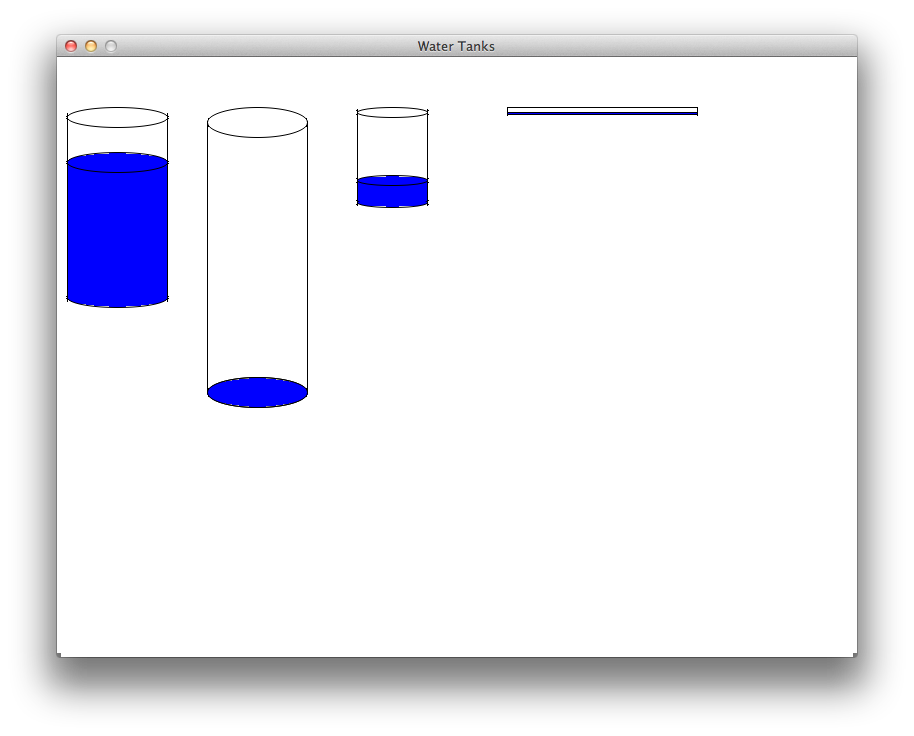
\includegraphics[width=0.7\textwidth]{./topics/storing-using-data/examples/WaterTank.png} 
   \caption{Example execution of the Water Tank program}
   \label{fig:water-tank-img}
\end{figure}

\clearpage

\csection{\ccode{clst:water-tank}{C Water Tank drawing code}{topics/storing-using-data/examples/water-tank.c}}

\csection{\ccode{clst:water-tank1}{C Water Tank drawing code (continued from \lref{clst:water-tank})}{topics/storing-using-data/examples/water-tank1.c}}

\passection{\pascode{lst:data-water-tank-pas}{Pascal Water Tank}{topics/storing-using-data/examples/WaterTank.pas}}

\passection{\pascode{lst:data-water-tank-1-pas}{Pascal Water Tank (continued from \lref{lst:data-water-tank-pas})}{topics/storing-using-data/examples/WaterTank1.pas}}

% subsubsection water_tank (end)


\clearpage
\subsection{Bicycle Race} % (fold)
\label{sub:bicycle_race}

The Bicycle Race program will simulate a thirty second sprint race between a number of bicycles. The race has a standing start, and then each racer accelerates as fast as they can for thirty seconds. The winner is the racer who makes it the furthest.

\begin{table}[h]
\centering
\begin{tabular}{l|p{10cm}}
  \hline
  \multicolumn{2}{c}{\textbf{Program Description}} \\
  \hline
  \textbf{Name} & \emph{Bike Race} \\
  \\
  \textbf{Description} & Calculates the position of seven bikes at the end of a timed race, drawing the final positions. Each bike's position is calculated based on a random acceleration over the duration of the race. \\
  \hline
\end{tabular}
\caption{Description of the Bike Race program}
\label{tbl:data-bike-race}
\end{table}


\begin{itemize}
  \item You can calculate distance the racers cover using Equation~\ref{eq:acceleration}.
  \begin{itemize}
    \item \emph{s} is the distance covered.
    \item \emph{u} is the starting speed
    \item \emph{t} is time.
    \item \emph{a} is acceleration.
  \end{itemize} 
  \begin{equation}
    s = ut + \frac{a t^2}{2}
    \label{eq:acceleration}
  \end{equation}
  \item This race has a standing start, so the initial speed of each racer will be 0.
  \item The time for the race is 30 seconds, this is constant.
  \item Each racer will have a randomly determined acceleration, with a maximum acceleration of 10 $pixels/second^2$
\end{itemize}

\begin{figure}[h]
   \centering
   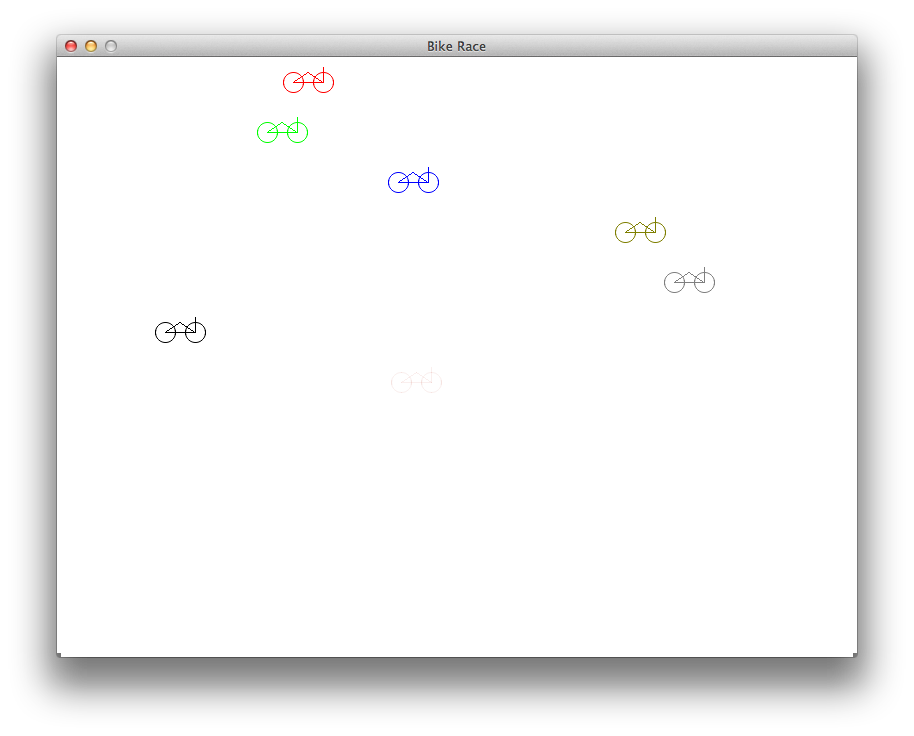
\includegraphics[width=0.6\textwidth]{./topics/storing-using-data/examples/BikeRace.png} 
   \caption{Example execution of the Bike Race program}
   \label{fig:bike-race-img}
\end{figure}

\csection{\ccode{clst:bike-race}{C Bicycle Race, continued in \lref{clst:bike-race1}}{topics/storing-using-data/examples/bike-race.c}}

\csection{\ccode{clst:bike-race1}{C Bicycle Race}{topics/storing-using-data/examples/bike-race1.c}}

\passection{\pascode{lst:bike-race-pas}{Pascal Bike Race)}{topics/storing-using-data/examples/BikeRace.pas}}

\passection{\pascode{lst:bike-race-1-pas}{Pascal Bike Race (continued from \lref{lst:bike-race-pas})}{topics/storing-using-data/examples/BikeRace1.pas}}

% subsection bicycle_race (end)

% \clearpage
% \subsection{Comet Orbit} % (fold)
% \label{sub:comet_orbit}
% 
% This program uses SwinGame to draw the orbit of the Hale-Bopp comet around the sun. The Hale-Bopp comet performs an elliptical orbit of the sun that can be plotted using Equation~ \ref{eq:orbit}. This equation calculates the radius (r) of the comet's position based on the \emph{angle} between the comet and the sun. Where \emph{e} is the Eccentricity value with a constant value of 0.995, and \emph{d} is the distance between the pole and directrix with a constant value of 1.828.
% 
% \begin{equation}
%   r = \frac{ed}{1 + e sin(angle)}
%   \label{eq:orbit}
% \end{equation}
% 
% \begin{table}[h]
% \centering
% \begin{tabular}{l|p{10cm}}
%   \hline
%   \multicolumn{2}{c}{\textbf{Program Description}} \\
%   \hline
%   \textbf{Name} & \emph{Comet Orbit} \\
%   \\
%   \textbf{Description} & Calculates and plots the position of the Hale-Bopp comet, based on an equation of its elliptical orbit of the sun. \\
%   \hline
% \end{tabular}
% \caption{Description of the Comet Orbit program}
% \label{tbl:data-comet-orbit}
% \end{table}
% 
% This will require functions and procedures to do the following:
% \begin{itemize}
%   \item A function to \textbf{calculate} the \textbf{r} value for the comet based on an \emph{angle}.
%   \item Functions to \textbf{convert} the \textbf{x} and \textbf{y} positions of the comet from AU (Astronomical Units) to pixel coordinates so that the comets position can be plotted on the screen.
%   \item A procedure to \textbf{Draw} the \textbf{comet} to the screen, based on its current angle.
%   \item A procedure to \textbf{Draw} the \textbf{sun}.
%   \item A procedure to \textbf{draw} the entire \textbf{system}, including the sun and the comet at a given angle.
%   \item The main procedure to coordinate actions (calling, draw system with different angle values).
% \end{itemize}
% 
% \clearpage
% 
% \csection{\ccode{clst:comet-orbit}{Comet Orbit, continued in \lref{clst:comet-orbit1}}{topics/storing-using-data/examples/comet-orbit.cpp}}
% 
% \begin{figure}[p]
% \csection{\ccode{clst:comet-orbit1}{Comet Orbit, continued in \lref{clst:comet-orbit2}}{topics/storing-using-data/examples/comet-orbit1.cpp}}
% \end{figure}
% 
% \begin{figure}[p]
% \csection{\ccode{clst:comet-orbit2}{Comet Orbit}{topics/storing-using-data/examples/comet-orbit2.cpp}}
% \end{figure}
% 
% % subsection comet_orbit (end)
